%%
%% This is file `sample-sigconf-authordraft.tex',
%% generated with the docstrip utility.
%%
%% The original source files were:
%%
%% samples.dtx  (with options: `all,proceedings,bibtex,authordraft')
%% 
%% IMPORTANT NOTICE:
%% 
%% For the copyright see the source file.
%% 
%% Any modified versions of this file must be renamed
%% with new filenames distinct from sample-sigconf-authordraft.tex.
%% 
%% For distribution of the original source see the terms
%% for copying and modification in the file samples.dtx.
%% 
%% This generated file may be distributed as long as the
%% original source files, as listed above, are part of the
%% same distribution. (The sources need not necessarily be
%% in the same archive or directory.)
%%
%%
%% Commands for TeXCount
%TC:macro \cite [option:text,text]
%TC:macro \citep [option:text,text]
%TC:macro \citet [option:text,text]
%TC:envir table 0 1
%TC:envir table* 0 1
%TC:envir tabular [ignore] word
%TC:envir displaymath 0 word
%TC:envir math 0 word
%TC:envir comment 0 0
%%
%% The first command in your LaTeX source must be the \documentclass
%% command.
%%
%% For submission and review of your manuscript please change the
%% command to \documentclass[manuscript, screen, review]{acmart}.
%%
%% When submitting camera ready or to TAPS, please change the command
%% to \documentclass[sigconf]{acmart} or whichever template is required
%% for your publication.
%%
%%
\documentclass[sigconf, 11pt]{acmart}
\usepackage{hyperref}
\usepackage{graphicx}
\graphicspath{ {./images/} }
\setcopyright{none}
\settopmatter{printacmref=false}
\renewcommand\footnotetextcopyrightpermission[1]{}
\pagestyle{plain}
\settopmatter{printfolios=true}
\acmConference{}{}{}

%%
%% end of the preamble, start of the body of the document source.
\begin{document}

%%
%% The "title" command has an optional parameter,
%% allowing the author to define a "short title" to be used in page headers.
\title{Use of Quantified Self to Reduce Bad Screentime Habits}


%%
%% The "author" command and its associated commands are used to define
%% the authors and their affiliations.
%% Of note is the shared affiliation of the first two authors, and the
%% "authornote" and "authornotemark" commands
%% used to denote shared contribution to the research.
\author{Logan Dube}
\email{dube@chalmers.se}
\affiliation{
  \institution{University of Newcastle / Chalmers University of Technology}
  \city{Newcastle}
  \country{Australia}
}

\author{Etienne}
\email{etienne.sandrard@chalmers.se}
\affiliation{
  \institution{CentraleSupélec/ Chalmers University of Technology}
  \city{Paris}
  \country{France}}

\author{Jacob Aaron Rossman}
\email{rossman@chalmers.se}
\affiliation{
  \institution{Nanyang Technological University / Chalmers University of Technology}
  \country{Singapore}}
  
\author{Zheng Wei}
\email{liau@chalmers.se}
\affiliation{
  \institution{Nanyang Technological University / Chalmers University of Technology}
  \country{Singapore}}

\author{Shan Hong Chua}
\email{shanho@student.chalmers.se}
\affiliation{
  \institution{Nanyang Technological University / Chalmers University of Technology}
  \country{Singapore}}


%%
%% The abstract is a short summary of the work to be presented in the
%% article.
\begin{abstract}
Globally, people average around 6 hours and 40 minutes of screen time per day. As for Gen Zs, they average around 9 hours of screen time per day (Duarte, 2025). This statistic is worrying given how these individuals are spending ¼ to ⅓ of their day on their phones. Studies show that excessive screen time is becoming more and more of a pressing issue with a myriad of problems that arise from it. These problems include an increased sedentary lifestyle as well as detrimental effects to physical health, mental health and overall well being. (Devi & Singh, 2023) Just to list a few, eye strain, shoulder pain, back pain, increased levels of depression, anxiety, mood disorders, impaired social relationships and cognitive development. The effects are reversed or minimised when the screen time is reduced (Griffiths et al., 2016) (Twenge, 2017).
\\

Screens are an unavoidable part of being a university student. From lecture halls to computer labs, screens are in constant view of students. However, the one screen that students can control the amount of time they look at is their phones. Yet, it remains to be the screen that students look at the most.
\\

In this report we conducted secondary research and primary surveys to gain knowledge about the target audience of university students, including their phone usage and their methods to reduce their screen time, if it is seen as a problem. In this preliminary research we found that university students are unaware of their screen time on a day-to-day and weekly basis and that they are unable to find ways to effectively reduce this. Based on these results, the group made a product of a “city building app” (City) to satisfy the needs of the target audience and reduce the contemporary problem of over-excessive screen usage in our society.
\\

In a bigger picture, people are increasingly becoming attached to screens and are unaware of this, which can damage mental and physical wellbeing. This report proposes a solution to this fact, building an application (City) which incentivises the reduction of time screen through a visual approach. This report and product hopes to make society more aware of the implications of excessive phone usage while providing a solution that can be integrated into everyday life.

\end{abstract}


\begin{teaserfigure}
  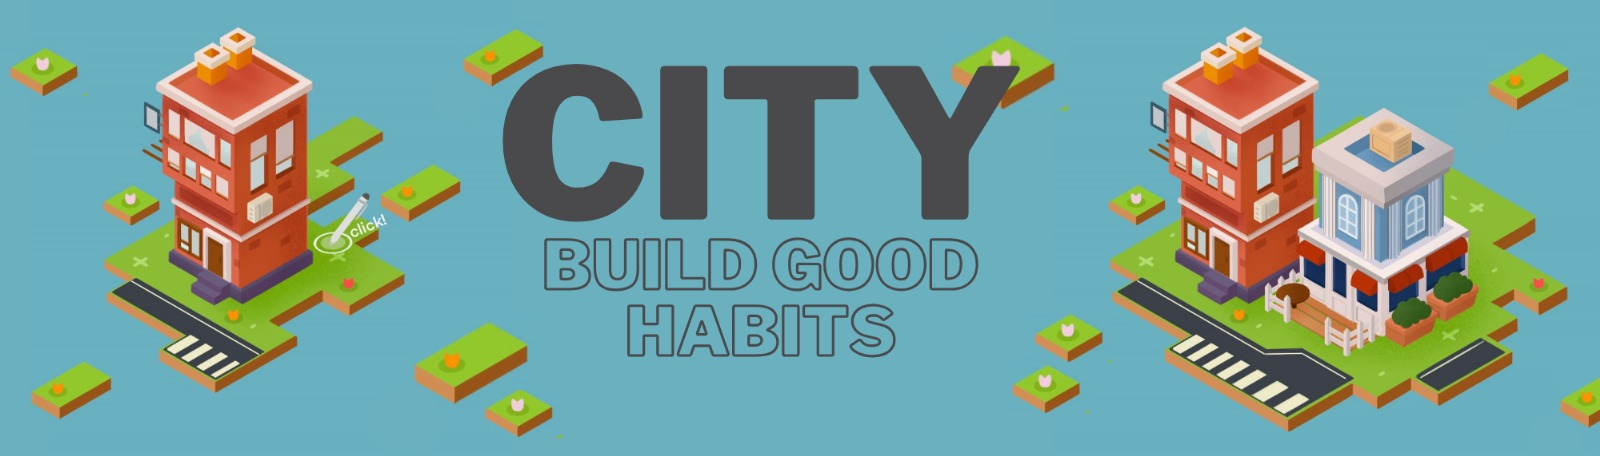
\includegraphics[width=\textwidth]{images/City Banner.jpg}
  \vspace{0.2}
\end{teaserfigure}

\maketitle


\section{Introduction}
In our research, we distributed 2 different surveys to achieve two different desired outcomes. The first survey was made to understand user needs and assessing how well our solution fits the problem described.The second survey was made to discover the design and usability of the product that is desired by end users
\\

We found that many students were not aware of the amount of time that they spend on their phone every day and that quite a number of them expressed astonishment over the results. On average, we found that the screen time usage could reach up to 9 hours per day.In fact, after the survey, some university students even shared, both personally or via messages,  that they could spend an entire day using their phones and doom scrolling streaming platforms like YouTube and Crunchyroll, social media sites like Facebook, TikTok and Instagram, or indulge in their mobile games. They even explained they just sit in one spot for the whole day and only get up for food or to use the toilet. There were also individuals that explained that they would start this process before daybreak until sunset and beyond that, sometimes not even noticing that it has gone dark outside. 
\\

A small number of university students did try to reduce their screen time after they read or heard about the benefits that it brings. However, many found themselves returning back to their original sedentary lifestyle. Some of them listed reasons like boredom and feeling sad without their devices. We believe that this may be a result of this habit being too ingrained in their lives and that they have overdosed on dopamine from their phones.
\\

The few university students that tried digital detox felt that they were ineffective or trying to achieve another purpose instead. There were mentions of an app to encourage less phone usage and ease them into a healthier amount of screen time. 
\\

Currently, phone usage data is locked behind many menu options making it virtually invisible to see. Additionally, the way the data is displayed in a day to day graph is meaningless as there is no explanation or insights of the data. Our project aims to make accessing information about your phone usage less troublesome as well as improve how this data is displayed. 
\\

As such, we have  decided to go in the direction of using a game to address this issue. This game would be a new take on the city building app genre. The main idea would be the less users use their phones, the more points they would gain that could help build their city. We took a bit of a counterintuitive approach as this approach is to do less to get more. This way, it would not feel like students are losing out but rather are gaining something by not doing the activity.
\\

It is important to note that the nature of the app is a contradiction as people have to use their phone to access the app. To clarify, the thought behind the app is that people will use their phone regardless and the app is simply a reminder and incentive for people not to use their phone.

\section{Related Work}
\subsection{Survey Results Contextualized}
Based on the Survey results we can observe and analyse:
\\

Most users are aware of how much they use their phone (70\% are aware - Figure I in Appendix) (Figure I in appendix). Additionally, General trend was user perception of phone usage much much lower than actual times used (only 20\% estimated phone usage of 6+ hours, reality is 75\% - from Figures II and III in Appendix).
\\

From the group of people surveyed, those who tried to reduce their screen usage did so in a restrictive way but found it was not sustainable (4 out of the 7 responses used a restrictive strategy and 3 out of 4 commented on its ineffectiveness - See survey results link in Appendix).
\\

For ideation of what people would like as a product, the survey demonstrated that majority of applicants found our idea of a “city building app” to be the most appealing idea (75\% - 15 out of 20 - From Figure IV). 15 out of 20 on Question 7 gave reasons for choosing the “city building app” such as it's a new fresh idea and 5/20 liked the idea of it seemingly like a game, yet it inhibits a different strategy and effect (See survey results link in Appendix).
\\

Finally, 90\% of users find it appealing to see visual progress instead of just numbers, statistics, graphs, etc (Figure V in Appendix)
\\

In summary, it is clearly apparent that users are unaware of the reality of screen usage and that they would like a product that would be incentive in a visual way, with the most desired product out of the options we have proposed being the “city building app”. From these results of the survey the group will pursue the idea of this app and the rest of the report is built from this product.

\subsection{Related Work}
In this paper, the related work will be discussed in terms of two different methods that previous products have employed to increase the wellbeing and healthy screen-time habits of their users.
\begin{enumerate}
    \item Phone locking apps: Apps that will restrict the use of some apps through an individual user-defined set of guidelines. For example, social media apps (such as Instagram) are able to be used for 45 mins and then the user is blocked from it for the rest of the day

    \item Subtle motivation: The use of subtle motivation employs a more user-friendly and seamless way of reducing screen-time. These apps employ strategies to promote but not force the user to do anything, supporting their own motivations. For example, daily affirmations, statistics and visuals that make the user excited about their improvement. 
\end{enumerate}

\subsubsection{Phone locking apps: “Screen Time” and “Get Off Your Phone”}
In comparison to Phone locking apps, our approach is widely different as we wanted to have the user have their own motivation and have a subtle push towards the stopping of phone addiction.
\\

In the experiment/study (Rahmillah et al., 2023) these phone locking apps gained a sentiment score of 70-78. A sentiment score is a qualitative evaluation given by users about how effective the product felt to them; a higher score means that the product was of better quality. This is good but comparatively, the sentiment score of other apps, that allowed for user control and promoted subtle improvement of habits, were much higher (Forest being the highest with 86\% sentiment). (Rahmillah et al., 2023).
\\

This higher sentiment score of Forest and other apps indicates that a pursuit of self improvement in terms of reducing screen time is more beneficial in the long run. When a strong restriction is imposed, it may be hard to change habits and often does not work. With individual desire to drive a change, university students can know how to slowly reduce their screen time since they understand themselves the best and know the causes behind their high app usage. 


\subsubsection{Forest: Focus for Productivity}
When we compare our app to the forest app, we see vast differences as our product focuses more on productivity than an active effort on reducing screen time as a whole, instead of as a short term study tool. Still, there are some similarities as it supports a change through visual feedback, not hard forcing or having numerical data. As such, our prototype will focus on recreating this effectiveness through subtlety.
As the phone locking apps are proven to not work and give user satisfaction, the product will follow closer to the ‘forest app’. Forest app is used for the studying and work habits, where a user would ‘plant a tree’ manually and then continue to have the application open for the duration that the tree grows. As this is a short term product whereby users are able to define the amount of time the tree takes to grow, this works for when a user wants to focus for a short term in hour-to-hour tasks. This clearly differs from our product as the app we wish to build will ‘build a city’ over a long period, focusing instead on improving screen time for long periods and day-to-day use.
\\

Forest app costs \$5.99 AUD (40 SEK), which is costly and deters the product, making it more exclusive. Due to our target audience being university students, it is more appropriate to make this application free. 
\\

Statistic: In the research study conducted on phone usage reducing apps (Forest was the most reviewed app (49.84\%) and had the highest positive sentiment (86\%)). (Rahmillah et al., 2023)


\subsection{Conclusive Statement:}
Based on online studies (Livanainen, 2023), Personal Quantification apps aforementioned have a dark side to them. It was found that tracking activities like daily steps, screen time or workouts can lead to an overemphasis on quantification and lead to adverse effects, despite them offering some benefits initially. By overly focusing on the amount of time spent on screens, individuals will experience less enjoyment from trying to improve themselves. In fact, there may be arising problems like increased stress and anxiety to maintain certain numbers consistently or to make the full use of their limited time on an app. Another revelation was that while screen time may be a good quantitative measure, we should also consider other aspects of well being that are less quantifiable. Over reliance on quantitative data might cause qualitative factors to be overlooked and ruin the effectiveness of a product as a whole.


\section{Design}
When designing our prototype, we first looked at our survey data and then determined the requirements, including functional and nonfunctional requirements. For functional requirements, we identified the scope of the product and knew that we wanted to create an app with a reward system through a game to help reduce screen time. The aim was to motivate users to cut down screen time and make screen time data more accessible due to the aforementioned issues of current measures. 

\subsection{Functional Requirements}
\subsubsection{Punishment Feature}
One functional requirement was to implement a punishment feature. B.F. Skinner's operant conditioning theory explains how behavior is shaped through reinforcement and punishment. While positive reinforcement (rewards) encourages desirable behaviors, punishment helps reduce unwanted behaviors by associating them with negative consequences. In the context of our app, the reward system involves building a thriving city as phone usage decreases, reinforcing positive behavior. However, without a punishment system, there is no deterrent for excessive phone use, making it less effective for behavior change.This design failed to account for users who do not feel strongly motivated by rewards alone. Without consequences for excessive phone use, users had no reason to reduce their screen time actively. They might lose interest in the app, as their city-building progress was not threatened by bad habits.This is supported by behavioral psychology research, which suggests that both reinforcement and punishment are necessary to shape lasting behavioral changes.
\\

\subsubsection{Personalized Approach}
Another functional requirement was to implement a more personalized approach One key piece of feedback we received on our first prototype was that the app treated screen time too generally, without distinguishing between different types of usage. Some days, screen time increased due to using YouTube for music, Google Maps for navigation, or FaceTime for family calls—activities that are far less harmful than doom scrolling. Our users wanted the app to better target problematic phone usage while avoiding penalties for justified screen time. The goal was to ensure that the phone remains a useful daily tool, rather than something they feel pressured to stop using entirely.To address this, we plan to implement a "missions" system that specifically targets overused apps like Instagram and TikTok, which are commonly seen as harmful. Additionally, users will have the ability to mark certain apps as problematic based on their own habits. This will make the experience more personalized and effective in helping users manage their screen time. These missions, which would involve reducing screen time, would grant access to new buildings for the user's city. For example, cutting screen time for Instagram, a high screen time app for the user, in half could unlock a reward. Difficulty levels could be introduced for these missions. A simple mission might be reducing usage by 30 minutes, while a more challenging one could be avoiding Instagram for an entire day. This system would make the experience more engaging while reinforcing healthier phone habits. For this mission system, we have also decided to make it a permanent feature given that the removal of a reward feature can diminish intrinsic motivation. These external rewards were found to shift the focus from internal satisfaction of reducing screen time to an external goal, making the activity feel more like work (Etkin, 2016).
\\

\subsubsection{Additional Functions}
Due to the iterative nature of the design process, we added more functional requirements over time. Another functional requirement was that we can add friends and see the castles of a few friends. Given this feature, users are able to bond with their peers as well as have more conversation starters which can help them get off their devices. Initially, we wanted to let users be able to view the castles of all their friends. However, we realised that this was counterintuitive to our goal of minimising screen time. This feature, if implemented, could have led to users spending a lot more time on this city building app than we desire. As such, we decided to have users only be able to view castles of a few of their friends instead. A related additional functional requirement was that each user can have a streak in which they achieve their daily tasks and that this streak can also be extended for friends whereby friends can have a friend streak together. Hasan et al. (2019) found that a gamified collaborative environment, through “leveling up, leaderboards and progress bars”, led to an improved student interaction with course contents as compared to a traditional learning environment. Allowing users to collaborate in completing certain tasks can help in fostering their sense of relatedness, thus motivating one another in achieving their goal of minimising screen time.
\\

\subsubsection{"Goals" to "Missions"}
Another small design implication that was changed was going from “Goals” to “Missions” (see Design 1 for “Goals” and Figure 4 for "Missions). The reasoning for the switch was that the group realised having a user define their own goals was counter-intuitive. This was due to two reasons:

\begin{enumerate}
    \item A user could set up an easy goal for a reward and therefore get the benefits of the app while not actually reducing their screen time habits
    \item Having users define their own goals would in turn keep them on their phone for longer as they have to create the goals on the app. Hence ruining the whole purpose of our design.
\end{enumerate}
Our choice to switch to missions was due to them being more generalised, automated and secure in guaranteeing that users use their phone less. Generalised problems such as “Spend x amount of time on Instagram today” (See Figure 1) prove to force users to get off their phone much more effectively than more specific tasks (e.g “Only open instagram 3 times today”). Further, the automation of the pre-defined goals was better as it means users cannot ‘cheat’ the app for rewards and also negates the use of the phone in setting up their own goals (For the implementation of this, See Figure 2).

\begin{figure}[h]
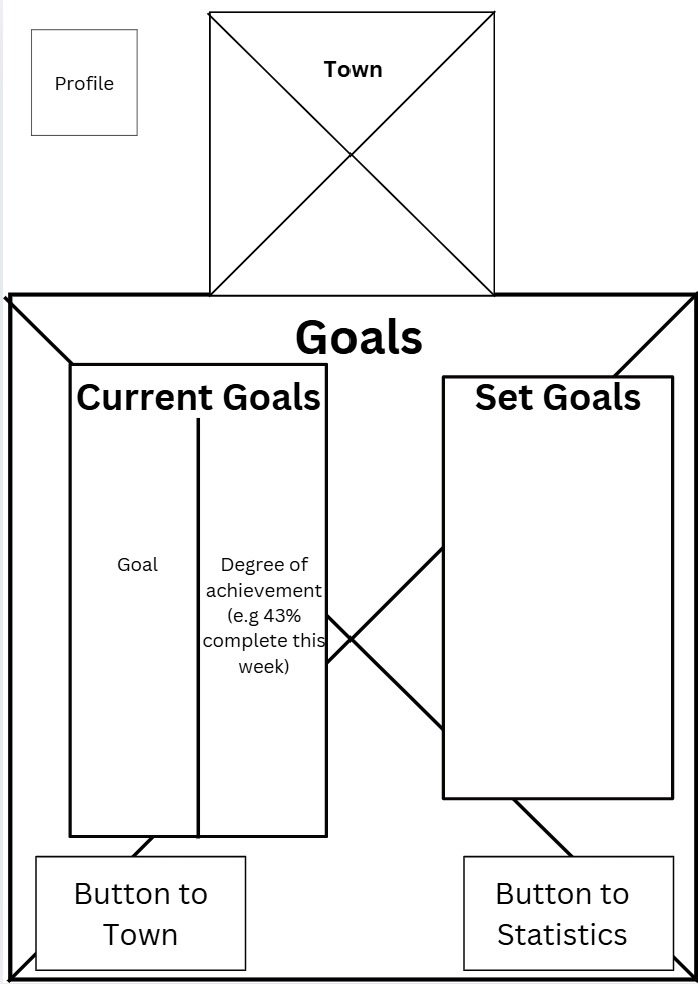
\includegraphics[width=2.5cm]{images/First Goals Design.jpg}
\caption{Initial Goals Page Wireframe}
\end{figure}

\subsection{Non-Functional Requirements}
Non Functional requirements were also considered in the creation of our prototype. This includes an inclusive design that caters to individuals of different backgrounds. On top of that, we aimed to cater to individuals with attention, visual disability. Given how our app has simple user interfaces made of bright colours, it helps to keep the attention of users. We have also implemented a colour changing feature and a zoom feature whereby individuals with color blindness and poor vision would not have trouble using our app. Apart from these, to make our app more inclusive, we even created a language preference page so that users can use the app in their preferred language.
\\

From these requirements, we proceeded to create iterations of a prototype, going from low to high fidelity.


\section{Implementation}

Our app is more of a high fidelity prototype. It focuses more on horizontal prototyping which demonstrates the entire feature spectrum without implementing them. We have done this through Genially which showcases the navigation of the user interface as well as the features of the app. Through it, we can determine accessibility and user preference of the app, be it functionality or user design. 
\\

In our app, we first made a wireframe of the app functionality to get an idea of how the app is structured and how it will turn out (See Figures 2, 3 and 4 for final design wireframe implementation). This was also due to how fast, cheap and easy it is to change the prototype. Afterwards, we consulted a personal friend to create high fidelity assets so that the user interface can look appealing and the app can be used for prototype surveying.  As of now, it is an interactive product which we built with Genially (Link found in Appendix).  

\begin{figure}[h]
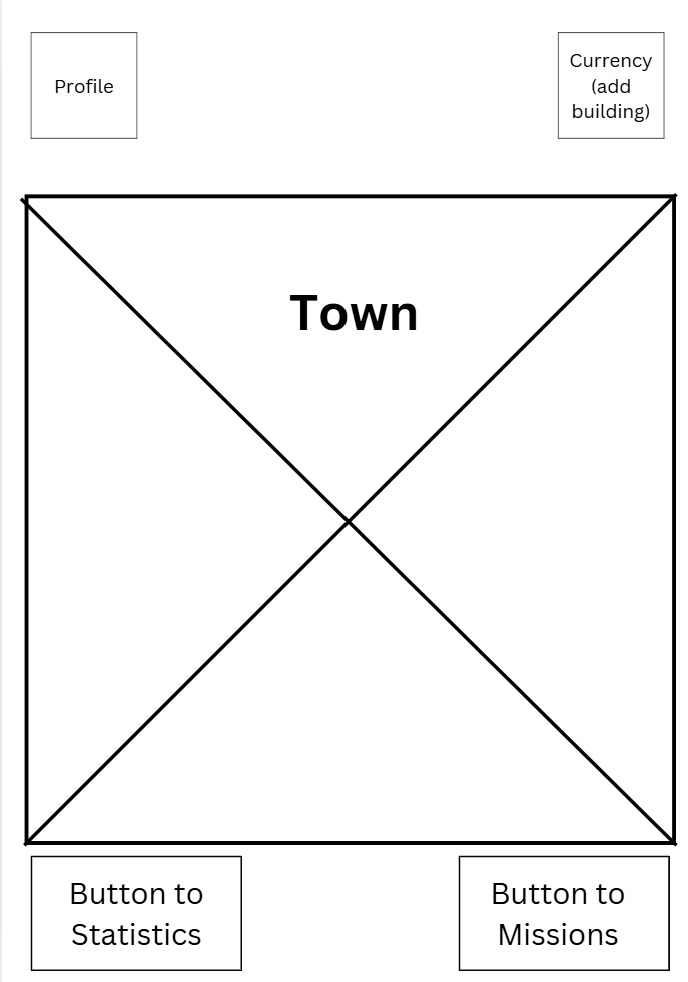
\includegraphics[width=2.5cm]{images/Second Town Design.jpg}
\caption{Final Town Page Wireframe}
\end{figure}

\begin{figure}[h]
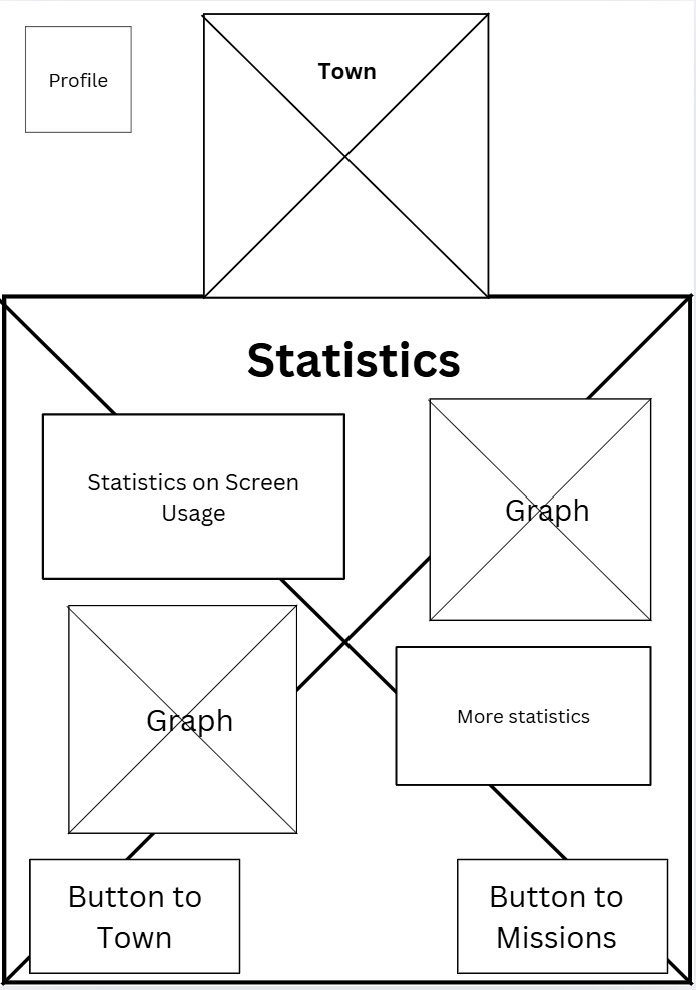
\includegraphics[width=2.5cm]{images/Second Statistic Design.jpg}
\caption{Final Statistics Page Wireframe}
\end{figure}

\begin{figure}[h]
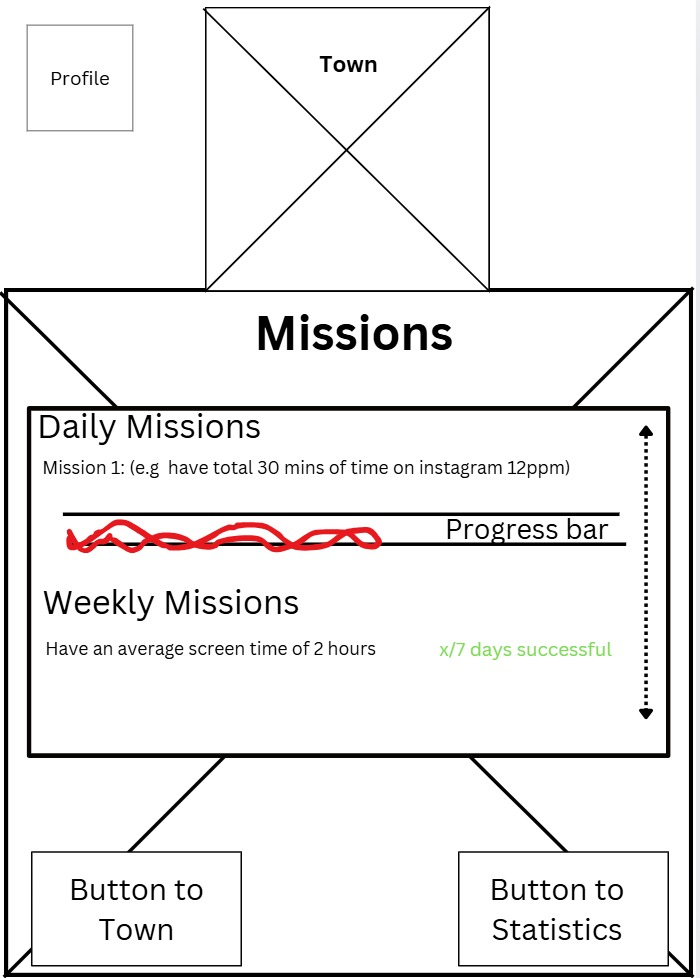
\includegraphics[width=2.5cm]{images/Second Missions Design.jpg}
\caption{Final Missions Page Wireframe}
\end{figure}


\section{Evaluation}
\subsection{Study Design}
In our study, we planned to determine how satisfied users would be when they use our application prototype. We decided to do a second survey to gather some quantitative data after users have used our prototype.
\\

It looks as described in the Design section. Alternative designs were dismissed as seen in the Design section. The main alternative design that was dismissed was the implementation of the feature whereby users can view the castles of all their friends. It was dismissed due to it being counterintuitive in getting users to reduce their screen time and an alternative design of only allowing users to view castles of some of their friends instead. 

\subsection{Participants}
For the sake of fairness, we conducted the study of our prototype on the same participants as our initial survey. This was done to ensure the independent variable remained constant so to reduce any external other factors affecting the results. Additionally, these participants would already have some context on the aim of our project.

\subsection{Apparatus}
Our study uses an indirect observation research method. This comes in the form of surveys and natural observations. Surveys are cheap and easy to do online, can reach a large group, garner feedback for a wide range of design characteristics and test varying levels of completeness. Also, it can help obtain numbers and statistics desired, fresh opinions to familiar design and catch design flaws in the real world. On top of this, our study uses naturalistic observation so that we can understand the context of use, and what and how people do what they do.
\\

Data is collected in the form of text via notes for naturalistic observation as well as survey results via Google forms.
\\

To run our prototype, we used Genially. We inserted the link to the prototype into the post prototype survey so they could easily answer feedback questions about the prototype right after they were done testing it. The participants saw the user interface of the prototype and the navigation between user interfaces. When the users start the app, they would see a screen with different buttons to the screen usage, missions and the ability to add buildings to the app. This screen also contains the current city’s buildings. In the screen usage screen, we display the statistics on screen time for different apps on a pie chart as well as a breakdown of screen time usage of apps on a bar chart with a range of very low to very high. In the missions screen, there is the city displayed at the top with daily and weekly missions.

\subsection{Procedure}
\subsubsection{Preparation}
To prepare for the study, we first defined the tasks. Even though our initial survey gave us the direction we should take with our project, we determined it was necessary to conduct more studies on our prototype to see if we were going in the right direction. After which, we recruited participants who are the same individuals for our initial survey. This keeps the independent variable as fair as possible, resulting in a more fair dependent variable result. Before carrying out the data collection, we distributed a consent form to all participants that states our purpose and the use of data. Then, we set up the test environment and conducted the study

\subsubsection{Conduction}
After developing the prototype, we gave participants a survey with the prototype. Throughout the conduct of the study, we motivated participants to think aloud as they performed tasks. Specifically, participants are to say what they are doing, looking at, wondering about, feeling and thinking. Observers are to observe what they do without answering any of the participant’s questions and note down all their observations. Participants are then to fill in the survey after using the prototype. Finally, we debrief the participants for final results.

\subsection{Results}
Most of our survey participants find our prototype design appealing (90\% - Figure VI in Appendix) and intuitive to use (80\% - Figure VII in Appendix). Majority agreed that the reward system is effective in encouraging users to reduce their screen time (80\% - Figure VIII in Appendix). However, regarding the effectiveness of a punishment system, the opinion is generally split with a slight majority of our respondents doubting its effectiveness (50\% - Figure IX in Appendix). As for collaborative features, most participants are receptive towards the implementation of this feature (70\% - Figure X in Appendix). Overall, 85\% of the participants are interested in using the app, with more than half stating that they will use it long-term (Figure XI in Appendix).


\section{Discussion}
\subsection{Ethical Concerns}
Our application, City, aims to reduce excessive screen time in a non restrictive and engaging manner. However, there are still some ethical concerns that need to be considered going forward with this. One major concern is the unintended psychological effects gamification strategies could bring. While effective, there is a chance that gamification results in a compulsion loop, where users become overly addicted to gaining rewards and building their virtual city rather than the aim of the app which is to reduce screen time for their personal well being (Statement supported by claim found in Etkin, 2016). Additionally, the app may become stressful for users as they feel pressured to not use their phone to maintain progress even when they actually need to access their phone. This could create unintended anxiety or guilt.
\\
On a more legal level, there are also always privacy and data security concerns. As the phone collects personal data like screen time, it is important to maintain transparency in data collection methods and usages. They should be compliant with international guidelines while offering opt-in or out settings to mitigate these risks even though opting-out would defeat the purpose of the application.
\\

\subsection{Social Impact}
While there are these ethical concerns that would need to be considered, we also believe the application could have a positive social impact on society. If widely adopted, our application could improve the digital well-being of students by helping them be more conscious and aware of their digital habits and to give them a push in the right direction of having healthier digital habits. Making screen time reduction an engaging and rewarding experience, social norms around using phones and excessive amounts could be changed, especially in universities where overuse is commonplace.
\\

\subsubsection{The Adversary Method}
We have a simple design with simple principles, so there are not many “dystopian” flaws. However, if the punishment feature were not implemented, a user who only wants to build their city — without actually reducing their screen time — could exploit the system. They could keep their screen on for extended periods using any random app on their phone, intentionally tricking City into detecting high phone usage. As a result, the app would suggest adapted missions, allowing the user to easily improve their city without engaging with the application as originally intended. That is an example of misuse, where our app could be perceived more as a game rather than a personal improvement tool. That’s mostly why we implemented this punishment feature, so people don’t want to come back to a high screen time. 
\\

In the design process, adversarial methods can involve creating apps that subtly exploit users for profit or manipulate their data. One such method is incorporating microtransactions, where the designer intentionally creates an app that offers a free service but includes numerous opportunities for users to spend money. This could be done through "pay-to-win" features, in-app purchases for virtual items, or by creating artificial barriers in the app that encourage users to spend money to progress.In the context of out project, a malicious designer may make it such that money might be spent to build more buildings and defeat the point of the app trying to reduce screen time. Designers with malicious intent may also hide these microtransactions behind engaging gameplay or features to create a sense of urgency or dependency, thereby extracting maximum revenue from users. In this case, the adversarial approach focuses on manipulating user behavior through psychological tactics, such as rewarding small purchases or creating addictive loops that lead users to spend more than they initially intended.
\\

Another adversarial design method involves collecting and selling user data without clear consent. In this scenario, the app may gather personal data, such as location, browsing habits, or contact information, under the guise of offering personalized services or improving user experience. The designer may embed data collection mechanisms deep within the app, making it difficult for users to opt-out or understand the extent of the information being gathered. Once the data is collected, it could be sold to third parties for targeted advertising, market research, or other profit-driven activities. This approach takes advantage of users’ trust, manipulating them into unknowingly agreeing to extensive data harvesting through convoluted privacy policies or hidden clauses in terms of service. By leveraging this information, malicious designers can generate significant revenue at the expense of user privacy, with little regard for ethical considerations or user protection.
\\

At a more macro level, 'City' could contribute to improving mental and physical health. Research source “Smartphone screen time reduction improves mental health: A randomized controlled trial - BMC medicine.” (Pieh et al., 2025) has shown that reduced screen time is linked to lower rates of mental conditions like depression or anxiety. We feel that if this app is successful it would help students feel more present in real-world interactions due to this lower level or stress or anxiety. However, we cannot deny the possibility that the opposite could happen due to this app. Peer pressure is a big potential danger to this app. If the app were to gain popularity, students who do not use it may feel peer pressured to use it even if they are not actively trying to reduce their screen time at the current moment or they already have healthy screen habits so adding this app could be a disservice to certain people. Additionally, students who struggle to reduce may feel frustrated at the lack of progress of their city, leading to more frustration.  


\subsection{Limitations}
Some limitations of our study include the limited sample size of our study. While the group was from a very diverse background, owing to the nature of being exchange students, it is still small and limits the generalizability of our findings to a broader population. While this app may seem effective in this limited sample size, it may work differently across a wider demographic.
\\

Another limitation is that the current prototype is a high-fidelity simulation rather than a fully functional application. While this allows us to test certain aspects like application flow, it is hard to test certain design concepts and functionality efficiently. 
\\

Lastly, our app is not able to differentiate when screen time is being used for positive uses like studying or communicating with friends or family. It generalizes all screen time as the same. 

\subsection{Future Works}
Given these limitations, there are several areas that future works would need to address. First would be expanding the user study. While our participants were all from the correct target audience, a much larger sample size would be necessary to see if our vision and aim would scale well to a much wider demographic as recruiting friends could have potential biases. Developing a functional prototype would also be a next step where real-time phone data is collected and integrated. This would allow us to observe and collect data about what users like about the app, what they find effective and other metrics that can tell us if we are going down the right path. Additionally, long time studies on this working prototype would help ascertain if our prototype was successful in fostering sustainable behaviour changes or if users revert once the novelty wears off. This would be easy to see just by tracking their screen time usage over time.

\section{Conclusion}
The City Builder application presents an innovative approach to reducing screen time by integrating gamification and social engagement. Through our research, we identified that users often lack awareness of their phone usage and find traditional screen-time tracking tools ineffective or uninspiring. By transforming the experience into an interactive and rewarding process, this app has the potential to motivate users to develop healthier digital habits.
\\

Our study's findings suggest that visual progress, personalized goals, and social competition are key motivators for behavior change. The next steps will focus on refining the app’s user experience, ensuring an optimal balance between user engagement and the original aim of reducing screen usage. With further iterations and testing, this concept can evolve into an effective tool for promoting mindful technology use, helping users take control of their screen time in a fun and rewarding way.


\newpage
\section{Use of AI Statement}

In the process of creating this report, we utilized the AI tool, ChatGPT, to assist in generating ideas, research, and enhancing clarity. Here's a detailed explanation of how these tools were employed and the value they added.
\\

One of the key ways ChatGPT was utilized in this report was during the initial brainstorming and outlining stages. We used ChatGPT to better understand the project topic.
\\

Furthermore, ChatGPT was used during the research process to find relevant information for the project. It provided a valuable resource for pulling together relevant information that might have otherwise required much more time spent combing through multiple sources or databases. For example, it pointed us to specific studies regarding excessive phone usage and existing solutions that tried to alleviate the issue. By summarizing key points and suggesting further exploration, ChatGPT streamlined the process and contributed to a well-rounded understanding of the topic.
\\

Additionally, we used a mix of Grammarly and ChatGPT in the refinement of sentences and paragraphs, enhancing the overall readability and professionalism of the report. We would often present drafts of sections and then ask for suggestions on how to improve specific aspects, such as sentence structure, word choice, or overall coherence. The tool’s ability to quickly generate alternative phrasing helped us to express our ideas and findings more clearly and effectively.
\\

For implementing the content into Latex (via Overleaf) and correctly formatting the report - including figures, text and references - ChatGPT was used. The purpose of using ChatGPT was to support the creation of the final report, making sure that the Latex syntax was correct and ensuring that implementation met the standards of a formal report.
\\

Overall, ChatGPT and other AI systems were used to support the creation of the report and product. During researching and initial brainstorming AI provided us with more clarity on the formal stages of research, information gathering and prototyping. AI was also used for the making of the report so that we could maintain professionalism and ensure that the content was to the best possible. All ideas, content and prototypes were made entirely by the members of the group, with AI helping in the processes. 

\section{References (ACM Format)}
Duarte, F. 2025. Alarming average screen time statistics (2024). Exploding Topics. https://explodingtopics.com/blog/screen-time-stats. 
\\

Devi, K.A. and Singh, S.K. 2023. The hazards of excessive screen time: Impacts on physical health, mental health, and overall well-being. Journal of education and health promotion. \\https://pmc.ncbi.nlm.nih.gov/articles/PMC10852174/. 

Griffiths, M.D., van Rooij, A.J., Kardefelt-Winther, D., et al. 2016. Working towards an international consensus on criteria for assessing internet gaming disorder: A critical commentary on petry et al. (2014). Addiction (Abingdon, England).
\\ https://pmc.ncbi.nlm.nih.gov/articles/PMC5699464/.
\\

Twenge, J.M. 2017. Increases in depressive symptoms, suicide-related outcomes, and suicide rates among U.S. adolescents after 2010 and links to increased new media screen time - Jean M. Twenge, Thomas E. Joiner, Megan L. Rogers, Gabrielle N. Martin, 2018. \\https://journals.sagepub.com/doi/full/10.1177/2167702617723376.\\


Etkin, J. 2016. The hidden cost of personal quantification. Journal of Consumer Research 42, 6, 967–984.
\\

Hasan, H.F., Nat, M. and Vanduhe, V.Z. (2019) ‘Gamified collaborative environment in Moodle’, IEEE Access, 7, pp. 89833–89844. doi:10.1109/access.2019.2926622.
\\

Iivanainen, R. 2023. The personal quantification bias: How tracking makes your life worse even when you choose it... Medium. https://riikkaiivanainen.medium.com/the-personal-quantification-bias-how-tracking-makes-your-life-worse-even-when-you-choose-it-14aadc664c9b.
\\

Rahmillah, F.I., Tariq, A., King, M., and  Oviedo-Trespalacios, O. 2023. Evaluating the effectiveness of apps designed to reduce mobile phone use and prevent maladaptive mobile phone use: Multimethod Study. Journal of medical Internet research.\\ 
https://pmc.ncbi.nlm.nih.gov/articles/PMC10498313/.
\\

Pieh, C., Humer, E., Hoenigl, A., et al. 2025. Smartphone screen time reduction improves mental health: A randomized controlled trial - BMC medicine. BioMed Central.\\ https://bmcmedicine.biomedcentral.com/articles/10.1186/s12916-025-03944-z.

\end{document}
